%-------------------------------------------------------------------------------
\section{Data Disguising}
%-------------------------------------------------------------------------------
\begin{figure}[t]
    \centering
    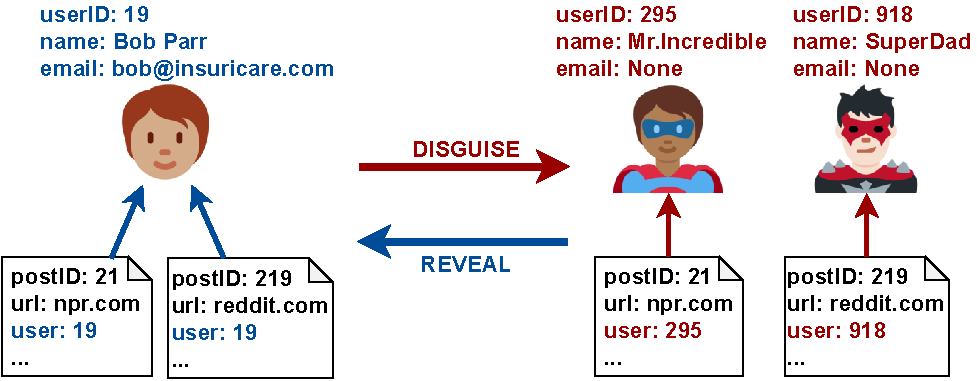
\includegraphics[width=0.47\textwidth]{img/disguises_new}

    \caption{Disguises move data (in this example, user Bob) from
             between different \emph{guises}. Guises represent the
             same data, but with different privacy properties (\eg
             anonymization).}
    \label{fig:example}
\end{figure}

%
We propose \emph{data disguising}, a systematic approach to privacy
transformations that separates them from application code.
%
Data disguising reasons about \emph{disguises}, privacy transformations that
follow an organized structure.
%
Disguises are based on the observation that application data can take
different forms, which we call \emph{guises}; some guises are identity-revealing while others are
privacy-preserving (to varying degrees).
%
%For example, a web application's database contents may assocate posts with
%an actual user as their author (an identity-revealing guise), or with
%one or more anonymous placeholder users (privacy-preserving guises).
%
A disguise transforms the database contents between these guises
(Figure~\ref{fig:example}).
%
%The structured nature of disguises allows a data disguising tool to
%automatically determine how to correctly compose multiple disguises, and to
%check that the end-state achieves the desired privacy properties.
%
%The tool uses the abstraction of \emph{per-user vaults}, which allow the tool to
%reintroduce destroyed data from prior disguises as necessary, while still ensuring that user data
%remains protected (\S\ref{sec:composition}).
%
%

%
An external data disguising tool reasons about and applies these disguises
based on the application's policy (a \emph{disguise specification}).
%
Application developers only need to invoke the tool's API to provide the
specification and to trigger individual disguises; the tool then performs the
necessary physical changes to the application's database.
%
These changes may include data removal, modification of contents, or
decorrelation by modifying references between objects.
%

\subsection{An Example Disguise}
\label{design:eg}
%
Consider disguising Bob when he deletes his HotCRP account.
%
Bob would prefer his papers and reviews to be unlinked from his identity.
%
HotCRP, on the other hand, would like to retain paper and review information that other users
find useful.
%
A developer can achieve both with disguises.
%A careful selection of edge and object transformations achieves both.
%

%
The application developer provides a specification of the disguise.
%
On applying the disguise, the tool unlinks Bob from his reviews via a
predicated transformation that reassign his reviews to individual, anonymous
placeholder users.
%
%This transforms Bob into one unique user guise per review.
%
The tool generates placeholder users with suitable default values; for
example, HotCRP users have a \texttt{disabled} attribute, and the tool sets
this for placeholder users, ensuring they have no permissions and cannot log
in.
%

%
Bob is further linked to papers through conflicts, which can
indicate co-authorship or a conflict of interest.
%
The disguise will not reassign these conflicts to the placeholder users,
since preserved conflicts could reidentify Bob as the likely author of a
review.
%
(As a trivial example of how this could work, consider that placeholder
users with identical conflict sets provide little decorrelation benefit.)
%
Instead, the disguise will remove Bob's conflicts.
%

%The disguise leaves all other edge types, ensuring that review and paper artifacts remain correctly
%linked: active reviewers still see the correct paper for their reviews, and active authors see the
%correct reviews for their papers, albeit potentially authored by anonymous, unlinkable guises of the
%original reviewer.
Unlike the current real-world HotCRP account deletion policy~\cite{hotcrp:privacy},
which deletes all objects belonging to Bob, this disguise strikes a balance between
decorrelating Bob's identity from his reviews and papers, and maintaining useful
information for other HotCRP users.
%
Furthermore, it is easy to imagine extending this disguise to automatically disguise
Bob after some time (\eg 2 years after the conference), protecting his future
research career by hiding his youthful reviewing sins.
%

%The tool disguises Bob when he invokes HotCRP account deletion.
%%
%Bob provides his secret key to decrypt and read from his vault, allowing the tool
%to retrieve and temporarily reverse any conflicting, reversible transformations
%that would make Bob's deletion fail: in particular, it recorrelates any
%of Bob's decorrelated paper conflicts and then properly removes them.
%%
%(Because the conflicts are removed, the decorrelation is not reapplied).
%%
%Bob wants his account deletion disguise to be reversible, so after performing the
%specified disguise updates, the tool records each transformation in the vault,
%re-encrypts the vault, and forgets the key.
